\begin{frame}[fragile]{Experiments: Performance}
    \begin{table}
        \centering
        \resizebox{\textwidth}{!}{
        \begin{tabular}{lcccccc}
            \toprule
            & \multicolumn{2}{c}{OvertPoly} & \multicolumn{2}{c}{OVERTVerify} & \multicolumn{2}{c}{CORA} \\ 
            \cmidrule(lr){2-3} \cmidrule(lr){4-5} \cmidrule(lr){6-7}
            & Time (s) & Volume & Time (s) & Volume &  Time (s) & Volume \\ 
            \midrule
            Single Pendulum &  $ \mathbf{1.6431} $ & $ \mathbf{5.533\textsc{e}{-2}} $ & $ 1.9232 $ & $ \mathbf{5.53\textsc{e}{-2}} $ & $ 2.919 $ & $ 7.6388 $ \\
            ACC &  $ \mathbf{23.1960} $ & $ \mathbf{3.819\textsc{e}{-3}} $ & $ 345.0036 $ & $ 1.119\textsc{e}{-2} $ & $ 25.4478 $ & $ 6.1596\textsc{e}{+5} $ \\
            TORA & $ \mathbf{1461.5640} $ & $ \mathbf{6.434\textsc{e}{-1}} $ & $ 13620.0628 $ & $ \mathbf{6.434\textsc{e}{-1}} $ & $ \times $ & $ 6.0325\textsc{e}{+2} $ \\
            Unicycle & $ \mathbf{7217.153} $ & $ \mathbf{8.979\textsc{e}{-6}} $ & $ 40109.9396 $ & $ 9.865\textsc{e}{-6} $ & $ \times $ & $ \times $ \\
            \bottomrule
        \end{tabular}}
        \caption{Benchmark computation time (s) and set volumes. Computation times listed for verified instances, and $ \times $ for unverified instances. All available set volumes listed. Best performance is highlighted in bold.}
        \label{tab:results}
    \end{table}
\end{frame}

\begin{frame}[fragile]{Experiments: Scalability}
    \begin{center}
        \begin{figure}
            \resizebox{0.6\textwidth}{!}{
            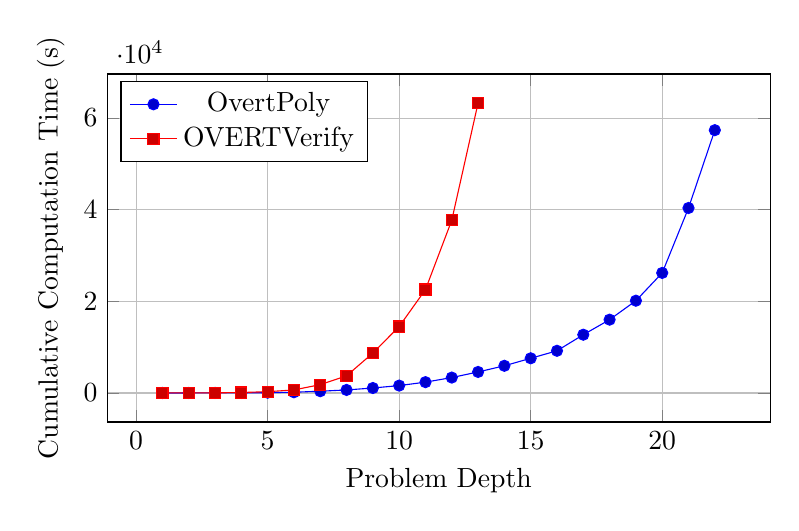
\begin{tikzpicture}
                \begin{axis}[
                    width=10cm,
                    height=6cm,
                    xlabel={Problem Depth},
                    ylabel={Cumulative Computation Time (s)},
                    grid=major,    % draws major grid lines
                    legend style={
                        at={(0.02,0.98)},
                        anchor=north west
                    }
                ]

                \addplot+[mark=*] coordinates {
                    (1, 0.139606)
                    (2, 1.20936)
                    (3, 5.954622)
                    (4, 18.516791)
                    (5, 62.81876)
                    (6, 156.655339)
                    (7, 379.155106)
                    (8, 656.64576)
                    (9, 1079.245311)
                    (10, 1607.974213)
                    (11, 2358.12396)
                    (12, 3357.880744)
                    (13, 4585.996028)
                    (14, 5929.248718)
                    (15, 7564.71484)
                    (16, 9201.581493)
                    (17, 12715.23366)
                    (18, 15998.02994)
                    (19, 20136.79328)
                    (20, 26202.32868)
                    (21, 40374.49559)
                    (22, 57361.10664)
                };
                \addlegendentry{OvertPoly}
                
                \addplot+[mark=square*] coordinates {
                    (1, 0.56439)
                    (2, 4.886867)
                    (3, 26.933899)
                    (4, 93.213138)
                    (5, 278.571822)
                    (6, 660.445473)
                    (7, 1812.827777)
                    (8, 3739.816229)
                    (9, 8711.381813)
                    (10, 14498.77977)
                    (11, 22566.04475)
                    (12, 37702.15095)
                    (13, 63285.72116)
                };
                \addlegendentry{OVERTVerify}
                
                \end{axis}
            \end{tikzpicture}
            }
            \caption{\footnotesize Pure symbolic reachability comparison between OverPoly and OVERTVerify using the Unicycle benchmark. Each tool was used used to compute as many pure symbolic reachable steps as possible with a (per optimizer call) timeout of $3600$ seconds.}
        \end{figure}
    \end{center}
\end{frame}

\begin{frame}[fragile]{Summary}
    \uncover<1->{
    We introduced OvertPoly, a combinatorial algorithm for forward reachability analysis of neural feedback systems.}

    \vspace{0.5cm}
    \uncover<2->{
        We demonstrated an \textbf{order of magnitude improvement} in performance compared to the current state-of-the-art.}
\end{frame}

\begin{frame}[fragile]
    \begin{center}
        \Huge Thank you!
    \end{center}
\end{frame}